\documentclass{beamer}
\usepackage[utf8]{inputenc}

\usetheme{Madrid}
\usecolortheme{beaver}

\title[About Beamer]{Sample Class on Beamer}
\subtitle{in sleepy mode}

\author[C.G. and A.B.]{Chris Gayle \inst{1} \\ A.~B.~De~Villiers\inst{2}}

\institute{
\inst{1}
Department of CSE\\
BUET\\
\inst{2}
Department of CSE\\
MIT
}

\date{\today}

\AtBeginSection[]{
\begin{frame}{We are going to see}
    \tableofcontents[currentsection]
\end{frame}
}

\begin{document}
\titlepage

\begin{frame}{Table of Contents}
\tableofcontents
    
\end{frame}
\section{Introduction}
\begin{frame}

\frametitle{Sample Frame}
    This is our first slide.
\end{frame}

\section{Animation}
\begin{frame}{Showing animation}
    \begin{enumerate}
        \item CSE 300 \pause
            \begin{itemize}
                \item So easy \pause
                \item Simple \pause
            \end{itemize}
        \item CSE 305
        \item CSE 310
    \end{enumerate}
    
\end{frame}


\begin{frame}{Showing animation in another way}
\setbeamercovered{dynamic}
    \begin{enumerate}
        \item<1-> CSE 300 
            \begin{itemize}
                \item<2-> So easy
                \item<3-> Simple
            \end{itemize}
        \item<4-> CSE 305
        \item<5-> CSE 310
    \end{enumerate}
    
\end{frame}

\begin{frame}{Table and Animation}
\setbeamercovered{dynamic}
\begin{center}
    \begin{tabular}{|c|c|c|}
        \hline
        Table & X & Y\\ 
        \hline
        A & \onslide<1->{1} & \onslide<2->{0}  \\
        \hline
        B & \onslide<3->{0} & \onslide<4->{1}  \\
        \hline
    \end{tabular}
\end{center}
    
\end{frame}

\section{Column}
\begin{frame}{Use of Columns and Images}
    \begin{columns}
        \column{0.5\textwidth}
        \begin{center}
    \begin{tabular}{|c|c|c|}
        \hline
        Table & X & Y\\ 
        \hline
        A & \onslide<1->{1} & \onslide<2->{0}  \\
        \hline
        B & \onslide<3->{0} & \onslide<4->{1}  \\
        \hline
    \end{tabular}
\end{center}  

\column{0.5\textwidth}
Simple description of the table.
    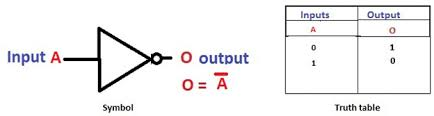
\includegraphics[height=1cm]{download.jpg}
    \end{columns}
\end{frame}

\section{Design}

\begin{frame}{Blocks}
    \begin{block}{Sample Block}
    This is a sample block.
    \end{block} 
    \begin{alertblock}{Sample Alert Block}
    This is a sample \textbf<2>{alert block}.
    \end{alertblock} 
    \begin{example}
    Sample \textcolor<3->{red}{example}.
    \end{example}
\end{frame}


\end{document}
